\section{Temporal Memory}
\label{sec:TM}
\subsection{Notation}
The sequence learning algorithm of the HTM theory is called the \textit{temporal memory} \cite{10.3389/fncir.2016.00023}. The temporal memory consists of a layer of $N$ mini-columns stacked vertically. Each mini-column contains $M$ number of HTM neurons, thus a total of $NM$ cells. The cells can be in one of three states; active, non-active, or predictive (depolarised). Thus, for a given time-step, $t$, the active cells in the layer are represented by the $M \times N$ binary matrix, $\boldsymbol{A}^{t}$, where $a^{t}_{ij}$ is the current active (non-active) state of the $i$'th cell in the $j$'th minicolumn \cite{10.3389/fncir.2016.00023}. For the same time-step, the predictive state of each cell is given by the $M \times N$ binary matrix, $\boldsymbol{\prod}^{t}$, of which the predictive state of the $i$'th cell in $j$'th minicolumn is denoted by $\pi^{t}_{ij}$ \cite{10.3389/fncir.2016.00023}.


Each cell in a layer has the potential to connect to any other cell via its basal dendrites. The set of basal dendritic segments of the $i$'th cell in $j$'th minicolumn is therefore represented by $\boldsymbol{D}_{ij}$. Each segment has a subset of $s$ potential synaptic connections from the $NM - 1$ cells in the layer. This subset is associated with a non-zero permanence value, where the $d$'th dendritic segment is represented as a $M \times N$ sparse matrix, $\boldsymbol{D}^{d}_{ij}$. A synaptic connection is only considered to be established if the permanence value is above a certain threshold. To represent these synapses with a weight of 1 on the same dendritic segment, we have the following $M \times N$ binary matrix, $\tilde{\boldsymbol{D}}^{d}_{ij}$ \cite{10.3389/fncir.2016.00023}.

\subsection{Initialisation of the Dendritic Segments}
With the initialisation of the network, each cell's dendritic segments are randomly assigned unique sets of $s$ potential synaptic connections. The non-zero permanence value of these connections is randomly initialised, with some being above the threshold and thus being connected, while others are not and therefore are unconnected \cite{10.3389/fncir.2016.00023}.

\subsection{Activation of Cells}
Each minicolumns feedforward receptive field is a subset of the entire feedforward pattern \cite{10.3389/fncir.2016.00023}. The receptive field of a minicolumn is shared by all cells in that minicolumn. A minicolumn becomes active if the number of synapses connected to the receptive field is above a certain threshold. However, there is an upper bound of $k$ minicolumns that can be active at the same time. Thus the minicolumns that have the highest number of active synapses get selected, which is also called the inhibitory process \cite{10.3389/fncir.2016.00023}. The set of $k$ winning minicolumns is denoted by $\boldsymbol{W}^{t}$. The active state of the individual cells in each minicolumn is computed by:


\begin{equation}
    a_{ij}^{t} =
    \begin{cases}
      1,&\text{if } j \in \boldsymbol{W}^{t} \text{ and } \pi^{t-1}_{ij} = 1\\
      1,&\text{if } j \in \boldsymbol{W}^{t} \text{ and } \sum_i\pi^{t-1}_{ij} = 0\\
      0,&\text{otherwise}
    \end{cases}
\end{equation}


In the first case the cell will become active if it was in a predictive state in the time-step before. In the second case, all cells in a minicolumn will become active if none of them previously where in a predictive state. If none of these cases applies, the cell will remain inactive \cite{10.3389/fncir.2016.00023}. Next, the predictive state of each cell in the winning column is computed as follows:


\begin{equation}
    \pi^{t}_{ij} = 
        \begin{cases}
            1,&\text{if } \exists_d\ \Big\| \tilde{\boldsymbol{D}}^{d}_{ij} \circ \boldsymbol{A}^{t} \Big\|_1 > \theta\\
            0,&\text{otherwise}
        \end{cases}
\end{equation}


For a cell to become depolarised in the current time-step, the contextual information received from the presynaptic input on any basal dendritic segment needs to be above the NMDA spike threshold, $\theta$. In order to detect if a segment is above this threshold, an element-wise multiplication, represented by $\circ$, of the dendritic segment and the active cells in the layer is computed. The $L_1$-norm of the result is then computed and compared with the threshold. In order for a cell to become depolarise, at least one segment needs to be active \cite{10.3389/fncir.2016.00023}.
 
\subsection{Learning of Dendritic Segments}
The reason a layer is able to learn multiple functionalities is due to the plasticity of the synapses belonging the cells \cite{10.3389/fncir.2016.00023}. In the HTM neuron, the updating rule for the permanence value of the synapses is a Hebbian-like rule. That is, if a cell was in a predictive state in a previous time-step, and then becomes active in the current because of the feedforward pattern, the synaptic connection that cause the depolarisation gets reinforced \cite{10.3389/fncir.2016.00023}. The segments responsible for the depolarisation are selected via the following operation:


\begin{equation}
    \label{eq:tm_predicted}
    \forall_{j\in\boldsymbol{W}^{t}}\ \Big( \pi^{t-1}_{ij} > 0 \Big) \text{ and } \Big\| \tilde{\boldsymbol{D}}^{d}_{ij} \circ \boldsymbol{A}^{t-1} \Big\|_1 > \theta
\end{equation}


First, the winning columns that had cells in a predictive state is selected. Next, the dendritic segments of these cells that cause the depolarisation is selected. However, if a winning column did not have cells in a predicted state, we need to reinforce the connection of the cell that had the most active segment. As this allows the cell to represent the transition of the sequence if it repeats later on \cite{10.3389/fncir.2016.00023}. To select the segment that where the most active, we first denote $\dot{\boldsymbol{D}^{d}_{ij}}$ as the $M \times N$ binary matrix of $\boldsymbol{D}^{d}_{ij}$, where each positive permanence value is represented as a 1 \cite{10.3389/fncir.2016.00023}. Next, we select the winning columns that did not have a cell in a predictive state, and then take the cell with the most active dendritic segment in each minicolumn.

\begin{equation}
    \label{eq:tm_close}
    \forall_{j\in\boldsymbol{W}^{t}}\ \Big( \sum_{i}\pi^{t-1}_{ij} = 0 \Big) \text{ and } \Big\| \tilde{\boldsymbol{D}}^{d}_{ij} \circ \boldsymbol{A}^{t-1} \Big\|_1 = max_i\Big(\Big\| \dot{\boldsymbol{D}}^{d}_{ij} \circ \boldsymbol{A}^{t-1} \Big\|_1 \Big)
\end{equation}


With the ability to select the relevant segments that cause a cell to become active, we now need to define the Hebbian-like learning rule, i.e. wire together fire together. That is, we reward connections with active presynaptic input, and punish the synapses that does not. To achieve this we decrease all permanence values by a small value $p^-$, while at the same time rewarding the connection with active presynaptic input by increasing them with a larger value $p^+$ \cite{10.3389/fncir.2016.00023}. 

\begin{equation}
    \label{eq:update_tm}
    \Delta \boldsymbol{D}^{d}_{ij} = p^+\Big(\dot{\boldsymbol{D}}^{d}_{ij} \circ \boldsymbol{A}^{t}\Big) - p^-\dot{\boldsymbol{D}}^{d}_{ij}
\end{equation}


As \autoref{eq:update_tm} only updates cells that became active, or closest to being active, selected by  \autoref{eq:tm_predicted} and \autoref{eq:tm_close} respectively, we need to define an equation for penalising the cells that did not become active \cite{10.3389/fncir.2016.00023}. The permanence values of these inactive cells will start to decay with a small value of $p^{--}$:

\begin{equation}
        \Delta \boldsymbol{D}^{d}_{ij} = p^{--}\dot{\boldsymbol{D}}^{d}_{ij} \text{ where } a_{ij}^t = 0 \text{ and } \Big\| \tilde{\boldsymbol{D}}^{d}_{ij} \circ \boldsymbol{A}^{t} \Big\|_1 > \theta
\end{equation}

Each cell is then updated with new permanence values for each of its dendritic segments by applying the following update rule:

\begin{equation}
    \boldsymbol{D}^{d}_{ij} = \boldsymbol{D}^{d}_{ij} + \Delta \boldsymbol{D}^{d}_{ij}
\end{equation}


As we have now gone through the temporal learning algorithm, we will now summarise this chapter. First, we introduced the HTM neuron and how it is modelled differently from the point neuron used in most ANNs. We then explained the properties of each dendritic segment of the HTM neuron. Then, we moved on to explaining how an HTM neuron learns to recognise input patterns. Next, we introduced the notion of sparse distributed representations (SDRs), which are binary vectors that represent information in an HTM network. With the familiarity of SDRs, we then went over the active processing property of the dendritic segment, and how each segment can detect multiple input patterns, i.e. with the \textit{union property}. Finally, we went over the algorithm for recognising temporal sequences in an HTM network and how it is able to learn to recognise new input patterns. 











\begin{comment}

\begin{figure}[H]
    \centering
    \scalebox{.4}{\input{background/HTM/tikz/minicol.tex}}
    \caption{Caption}
    \label{fig:my_label}
\end{figure}

\begin{figure}[H]
    \centering
    \scalebox{.2}{\centering
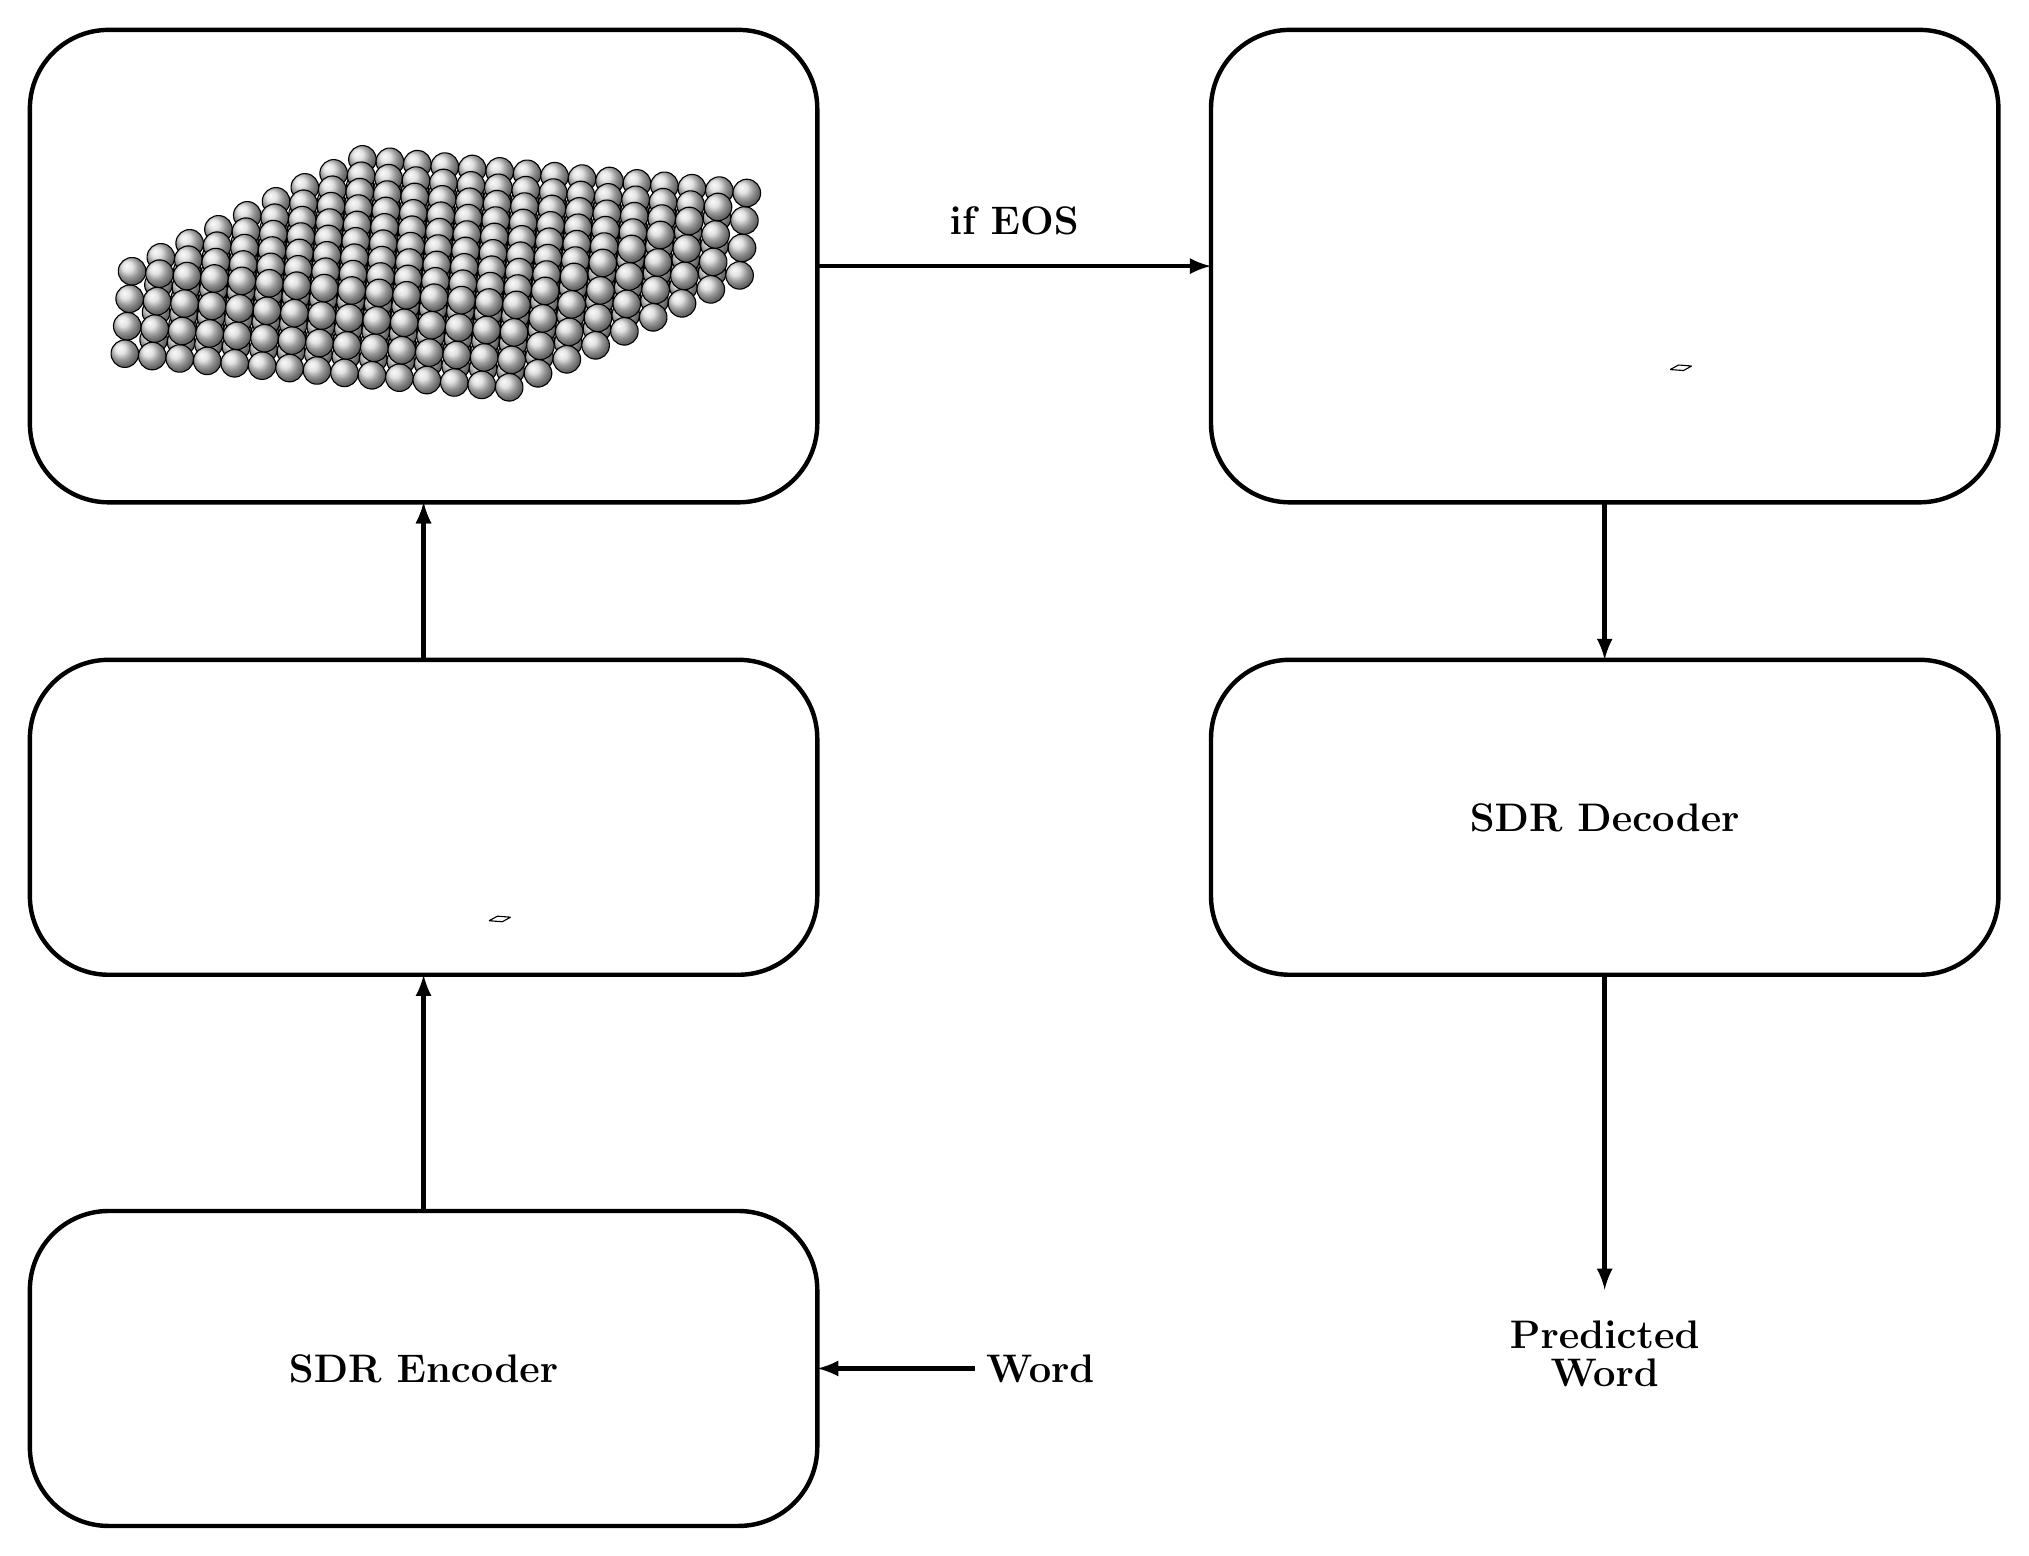
\begin{tikzpicture}



\draw[-latex,ultra thick] (6,-12) to node [right=1cm] {\Large\textbf{Word}} (4,-12);

\draw [rounded corners=1cm,ultra thick] (-6,-14) rectangle ++(10,4) node [midway] {\Large\textbf{SDR Encoder}};


\draw[-latex,ultra thick](-1,-10) to (-1,-7);



\draw [rounded corners=1cm,ultra thick] (-6,-7) rectangle ++(10,4) node [midway] {};
\begin{scope}[yshift=-180,yslant=.55,xslant=-1.6,scale=0.105]
        \ColorCells
        \draw (0, 0) grid (\GridSize, \GridSize);
        \coordinate (input);
\end{scope}

\draw[-latex,ultra thick](-1,-3) to (-1,-1);


\draw [rounded corners=1cm,ultra thick] (9,-1) rectangle ++(10,6) node [midway] {};
\begin{scope}[xshift=15cm, yshift=7cm, yshift=-180, yslant=.55, xslant=-1.6, scale=0.105] 
    \ColorCells
    \draw (0, 0) grid (\GridSize, \GridSize);
    \coordinate (output);
\end{scope}  


\draw[-latex,ultra thick](-1,-3) to (-1,-1);

\draw[-latex,ultra thick] (4,2) to node [above=.25cm] {\Large\textbf{if EOS}} (9,2);


\draw[-latex,ultra thick](14,-1) to (14,-3);

\draw [rounded corners=1cm,ultra thick] (9,-7) rectangle ++(10,4) node [midway] {\Large\textbf{SDR Decoder}};


\draw[-latex,ultra thick] (14,-7) to node [below=2.25cm] {\begin{tabular}{c} \Large\textbf{Predicted} \\ \Large\textbf{Word} \end{tabular}} (14,-11);


\draw [rounded corners=1cm,ultra thick] (-6,-1) rectangle ++(10,6) node [midway] {};

\begin{scope}[rotate around = {-5:(0,20,20)}, yshift=2.5cm,xshift=-0.5cm,scale=0.7]
   
    \foreach \x  in {0.75,1.25,1.75,2.25,2.75,3.25,3.75,4.25,4.75,5.25,5.75,6.25,6.75,7.25,7.75}%
        \shadedraw [ball color= gray!30] (\x,2,1.55*2.5) circle (0.25cm);
    \foreach \x  in {0.75,1.25,1.75,2.25,2.75,3.25,3.75,4.25,4.75,5.25,5.75,6.25,6.75,7.25,7.75}%
        \shadedraw [ball color= gray!30] (\x-.2,2,1.55*3) circle (0.25cm);
    \foreach \x  in {0.75,1.25,1.75,2.25,2.75,3.25,3.75,4.25,4.75,5.25,5.75,6.25,6.75,7.25,7.75}%
        \shadedraw [ball color= gray!30] (\x-.4,2,1.55*3.5) circle (0.25cm);
    \foreach \x  in {0.75,1.25,1.75,2.25,2.75,3.25,3.75,4.25,4.75,5.25,5.75,6.25,6.75,7.25,7.75}%
        \shadedraw [ball color= gray!30] (\x-.6,2,1.55*4) circle (0.25cm);
    \foreach \x  in {0.75,1.25,1.75,2.25,2.75,3.25,3.75,4.25,4.75,5.25,5.75,6.25,6.75,7.25,7.75}%
        \shadedraw [ball color= gray!30] (\x-.8,2,1.55*4.5) circle (0.25cm);
    \foreach \x  in {0.75,1.25,1.75,2.25,2.75,3.25,3.75,4.25,4.75,5.25,5.75,6.25,6.75,7.25,7.75}%
        \shadedraw [ball color= gray!30] (\x-1,2,1.55*5) circle (0.25cm);
    \foreach \x  in {0.75,1.25,1.75,2.25,2.75,3.25,3.75,4.25,4.75,5.25,5.75,6.25,6.75,7.25,7.75}%
        \shadedraw [ball color= gray!30] (\x-1.2,2,1.55*5.5) circle (0.25cm);
    \foreach \x  in {0.75,1.25,1.75,2.25,2.75,3.25,3.75,4.25,4.75,5.25,5.75,6.25,6.75,7.25,7.75}%
        \shadedraw [ball color= gray!30] (\x-1.4,2,1.55*6) circle (0.25cm);
    \foreach \x  in {0.75,1.25,1.75,2.25,2.75,3.25,3.75,4.25,4.75,5.25,5.75,6.25,6.75,7.25,7.75}%
        \shadedraw [ball color= gray!30] (\x-1.6,2,1.55*6.5) circle (0.25cm);


    \foreach \x  in {0.75,1.25,1.75,2.25,2.75,3.25,3.75,4.25,4.75,5.25,5.75,6.25,6.75,7.25,7.75}%
        \shadedraw [ball color= gray!30] (\x,2.5,1.55*2.5) circle (0.25cm);
    \foreach \x  in {0.75,1.25,1.75,2.25,2.75,3.25,3.75,4.25,4.75,5.25,5.75,6.25,6.75,7.25,7.75}%
        \shadedraw [ball color= gray!30] (\x-.2,2.5,1.55*3) circle (0.25cm);
    \foreach \x  in {0.75,1.25,1.75,2.25,2.75,3.25,3.75,4.25,4.75,5.25,5.75,6.25,6.75,7.25,7.75}%
        \shadedraw [ball color= gray!30] (\x-.4,2.5,1.55*3.5) circle (0.25cm);
    \foreach \x  in {0.75,1.25,1.75,2.25,2.75,3.25,3.75,4.25,4.75,5.25,5.75,6.25,6.75,7.25,7.75}%
        \shadedraw [ball color= gray!30] (\x-.6,2.5,1.55*4) circle (0.25cm);
    \foreach \x  in {0.75,1.25,1.75,2.25,2.75,3.25,3.75,4.25,4.75,5.25,5.75,6.25,6.75,7.25,7.75}%
        \shadedraw [ball color= gray!30] (\x-.8,2.5,1.55*4.5) circle (0.25cm);
    \foreach \x  in {0.75,1.25,1.75,2.25,2.75,3.25,3.75,4.25,4.75,5.25,5.75,6.25,6.75,7.25,7.75}%
        \shadedraw [ball color= gray!30] (\x-1,2.5,1.55*5) circle (0.25cm);
    \foreach \x  in {0.75,1.25,1.75,2.25,2.75,3.25,3.75,4.25,4.75,5.25,5.75,6.25,6.75,7.25,7.75}%
        \shadedraw [ball color= gray!30] (\x-1.2,2.5,1.55*5.5) circle (0.25cm);
    \foreach \x  in {0.75,1.25,1.75,2.25,2.75,3.25,3.75,4.25,4.75,5.25,5.75,6.25,6.75,7.25,7.75}%
        \shadedraw [ball color= gray!30] (\x-1.4,2.5,1.55*6) circle (0.25cm);
    \foreach \x  in {0.75,1.25,1.75,2.25,2.75,3.25,3.75,4.25,4.75,5.25,5.75,6.25,6.75,7.25,7.75}%
        \shadedraw [ball color= gray!30] (\x-1.6,2.5,1.55*6.5) circle (0.25cm);


    \foreach \x  in {0.75,1.25,1.75,2.25,2.75,3.25,3.75,4.25,4.75,5.25,5.75,6.25,6.75,7.25,7.75}%
        \shadedraw [ball color= gray!30] (\x,3,1.55*2.5) circle (0.25cm);
    \foreach \x  in {0.75,1.25,1.75,2.25,2.75,3.25,3.75,4.25,4.75,5.25,5.75,6.25,6.75,7.25,7.75}%
        \shadedraw [ball color= gray!30] (\x-.2,3,1.55*3) circle (0.25cm);
    \foreach \x  in {0.75,1.25,1.75,2.25,2.75,3.25,3.75,4.25,4.75,5.25,5.75,6.25,6.75,7.25,7.75}%
        \shadedraw [ball color= gray!30] (\x-.4,3,1.55*3.5) circle (0.25cm);
    \foreach \x  in {0.75,1.25,1.75,2.25,2.75,3.25,3.75,4.25,4.75,5.25,5.75,6.25,6.75,7.25,7.75}%
        \shadedraw [ball color= gray!30] (\x-.6,3,1.55*4) circle (0.25cm);
    \foreach \x  in {0.75,1.25,1.75,2.25,2.75,3.25,3.75,4.25,4.75,5.25,5.75,6.25,6.75,7.25,7.75}%
        \shadedraw [ball color= gray!30] (\x-.8,3,1.55*4.5) circle (0.25cm);
    \foreach \x  in {0.75,1.25,1.75,2.25,2.75,3.25,3.75,4.25,4.75,5.25,5.75,6.25,6.75,7.25,7.75}%
        \shadedraw [ball color= gray!30] (\x-1,3,1.55*5) circle (0.25cm);
     \foreach \x  in {0.75,1.25,1.75,2.25,2.75,3.25,3.75,4.25,4.75,5.25,5.75,6.25,6.75,7.25,7.75}%
        \shadedraw [ball color= gray!30] (\x-1.2,3,1.55*5.5) circle (0.25cm);
    \foreach \x  in {0.75,1.25,1.75,2.25,2.75,3.25,3.75,4.25,4.75,5.25,5.75,6.25,6.75,7.25,7.75}%
        \shadedraw [ball color= gray!30] (\x-1.4,3,1.55*6) circle (0.25cm);
    \foreach \x  in {0.75,1.25,1.75,2.25,2.75,3.25,3.75,4.25,4.75,5.25,5.75,6.25,6.75,7.25,7.75}%
        \shadedraw [ball color= gray!30] (\x-1.6,3,1.55*6.5) circle (0.25cm);
    
    
    
    \foreach \x  in {0.75,1.25,1.75,2.25,2.75,3.25,3.75,4.25,4.75,5.25,5.75,6.25,6.75,7.25,7.75}%
        \shadedraw [ball color= gray!30] (\x,3.5,1.55*2.5) circle (0.25cm);
    \foreach \x  in {0.75,1.25,1.75,2.25,2.75,3.25,3.75,4.25,4.75,5.25,5.75,6.25,6.75,7.25,7.75}%
        \shadedraw [ball color= gray!30] (\x-.2,3.5,1.55*3) circle (0.25cm);
    \foreach \x  in {0.75,1.25,1.75,2.25,2.75,3.25,3.75,4.25,4.75,5.25,5.75,6.25,6.75,7.25,7.75}%
        \shadedraw [ball color= gray!30] (\x-.4,3.5,1.55*3.5) circle (0.25cm);
    \foreach \x  in {0.75,1.25,1.75,2.25,2.75,3.25,3.75,4.25,4.75,5.25,5.75,6.25,6.75,7.25,7.75}%
        \shadedraw [ball color= gray!30] (\x-.6,3.5,1.55*4) circle (0.25cm);
    \foreach \x  in {0.75,1.25,1.75,2.25,2.75,3.25,3.75,4.25,4.75,5.25,5.75,6.25,6.75,7.25,7.75}%
        \shadedraw [ball color= gray!30] (\x-.8,3.5,1.55*4.5) circle (0.25cm);
    \foreach \x  in {0.75,1.25,1.75,2.25,2.75,3.25,3.75,4.25,4.75,5.25,5.75,6.25,6.75,7.25,7.75}%
        \shadedraw [ball color= gray!30] (\x-1,3.5,1.55*5) circle (0.25cm);
    \foreach \x  in {0.75,1.25,1.75,2.25,2.75,3.25,3.75,4.25,4.75,5.25,5.75,6.25,6.75,7.25,7.75}%
        \shadedraw [ball color= gray!30] (\x-1.2,3.5,1.55*5.5) circle (0.25cm);
    \foreach \x  in {0.75,1.25,1.75,2.25,2.75,3.25,3.75,4.25,4.75,5.25,5.75,6.25,6.75,7.25,7.75}%
        \shadedraw [ball color= gray!30] (\x-1.4,3.5,1.55*6) circle (0.25cm);
    \foreach \x  in {0.75,1.25,1.75,2.25,2.75,3.25,3.75,4.25,4.75,5.25,5.75,6.25,6.75,7.25,7.75}%
        \shadedraw [ball color= gray!30] (\x-1.6,3.5,1.55*6.5) circle (0.25cm); 
\end{scope}
\end{tikzpicture}}
    \caption{Caption}
    \label{fig:my_label}
\end{figure}
\end{comment}

